%Chapter 8

\chapter{System Performance Evaluation} % Main chapter title

\label{eval} % For referencing the chapter elsewhere, use \ref{eval} 

\lhead{System Performance Evaluation. \emph{System Performance Evaluation}} % This is for the header on each page - perhaps a shortened title
%----------------------------------------------------------------------------------------
In this chapter we present our system\'s performance evaluation and performance analysis. However, we need to stress again on the lack of resource for Arabic language and how that caused performance degradation of some components of the system. The chapter is organized as follows; resources are discussed from the performance point-of-view in section ~\ref{sec:challenges}, used performance measures are explained in section ~\ref{sec:tech}, while the design of the test cases is explained in section ~\ref{sec:test}. Finally, the obtained results are viewed in the last section of the chapter section ~\ref{sec:results}.

\section{Challenges}\label{sec:challenges}
This is section we give an overall discussion of the resources for Arabic language and its limitations from the perspective of performance. The main components of our system are Web Crawlers, Pre-processing tools, Similarity measure, Clustering algorithms and Recommender System. \\
We used Web Harvest as our web crawler which surfs some given URL domains and retrieves web pages\' content. Web Harvest has a good performance and a plausible throughput given the number of web pages that were crawled. \\For the Pre-processing part we used Stanford\'s POS which gave a very good performance for Arabic language. We also used different Stemmers, light stemmer like the Arabic stemmer used by Lucene. However, we also used El-Khoga stemmer as different type of stemmer. All the Pre-processing components gave a plausible output and could scale-up to processing thousands of documents.\\ 
For the Similarity part, we examined different approaches; Lexical, Knowledge-based and Corpus-based similarities. For Lexical similarity, we used Lucene to build inverted index on the retrieved documents and calculate the TF-IDF. \\
Lucene is proved to be highly optimized and it gave a very good performance with processing Arabic text. For Knowledge-based approach, first we tried Arabic WordNet (AWN) to model the concepts and the knowledge of the Arabic language. \\
Unfortunately, AWN was a performance bottleneck in our system. The running time of AWN resulted in a significant degradation in the system\'s performance. AWN could not scale-up to handle large data-sets. Wikipedia as ontology was our alternative to AWN. Wikipedia approach was very promising when compared to AWN, but, due to time constraints, we could not investigate this new approach as much as we did with the AWN approach. The Wikipedia approach scaled-up to relatively large data-sets of documents and allowed us to compute hundreds of thousands of documents similarities. Indeed, Wikipedia wasn\'t computationally expensive when compared to AWN. 
Another resource that affected our performance evaluation process was the existence of a labeled training set for Arabic language. Another thing was that, we had to run the web crawlers on News websites as it\'s almost the only on-line content that is written in formal Arabic language. \\

Although Arabic language is used by more than $330$ million Arabic speakers, there are few systems that we can compare our system with, also there are no human-judged dataset for Arabic text. We used Aljazeera data set \footnote[1]{Available online at http://filebox.vt.edu/users/dsaid/AljNews.tar.gz} that is categorized in to $8$ categories to measure the accuracy of the different clustering algorithms.

Due to all the previously explained issues, with the addition of our hardware resources� capabilities and the wide set of alternatives to almost each of the system�s components, we were limited by a few number of experiments. A single run might take more than 12 hours to produce an output. These, previously mentioned, reasons also limited our ability to run the clustering algorithms like Mitosis and DBSCAN with a wide range of parameters� values to be able to tune the algorithms with the best parameter set.\\
However, we were able to test the whole system on two different randomly selected data-sets. The data-set was collected from Aljazeera news website. Some of the system techniques were tested on three different data-sets. We examined, as large as possible, different ranges of parameters for the Mitosis clustering algorithm. We also considered different performance measures like Purity and Confusion Matrix.\\


\section{Evaluation techniques}\label{sec:tech}
We chose to evaluate the performance of the system by evaluating the performance of the clustering algorithms. We tested every component of the system individually before integrating it with the other system components. However, many test runs were conducted to evaluate the overall system, which was achieved by evaluating the clustering algorithm. We also chose Purity and Confusion Matrix as performance measure techniques. In this section we will discuss the performance measurement technique that we used. \\
The cluster hypothesis states the fundamental assumption we make when using clustering in information retrieval,\textit{"Documents in the same cluster behave similarly with respect to relevance to information needs."} The hypothesis states that if there is a document from a cluster that is relevant to a search request, then it is likely that other documents from the same cluster are also relevant. This is because clustering puts together documents that share many terms.\\
Typical objective functions in clustering formalize the goal of attaining high intra-cluster similarity (documents within a cluster are similar) and low inter-cluster similarity (documents from different clusters are dissimilar). This is an internal criterion for the quality of a clustering. But good scores on an internal criterion do not necessarily translate into good effectiveness in an application. An alternative to internal criteria is direct evaluation in the application of interest. For search result clustering, we may want to measure the time it takes users to find an answer with different clustering algorithms. This is the most direct evaluation, but it is expensive, especially if large user studies are necessary.\\
As a surrogate for user judgments, we can use a set of classes in an evaluation benchmark or gold standard. The gold standard is ideally produced by human judges with a good level of inter-judge agreement. We can then compute an external criterion that evaluates how well the clustering matches the gold standard classes.\\

\subsection{Purity}
This section introduces external criterion of clustering quality. Purity is a simple and transparent evaluation measure. To compute Purity, each cluster is assigned to the class which is most frequent in the cluster, and then the accuracy of this assignment is measured by counting the number of correctly assigned documents and dividing by N.
Formally:
\begin{equation}
Purity(\omega,C) =\frac{1}{N}\sum_k max_j|w_k \cap c_j|
\end{equation}
Where $\omega= \{w_1,w_2,�,w_K \}$  is the set of clusters,  $C= \{c_1,c_2,�,c_J \}$ is the set of classes and N is the total number of documents. We interpret $w_k$ as the set of documents in $w_k$ and $c_j$ as the set of documents $inc_j$. We present an example of how to compute purity in Figure ~\ref{fig:purityFig}. Bad clustering has purity values close to 0; a perfect clustering has a purity of 1. High purity is easy to achieve when the number of clusters is large - in particular, purity is 1 if each document gets its own cluster.
\begin{figure}[htbp]
	\centering
		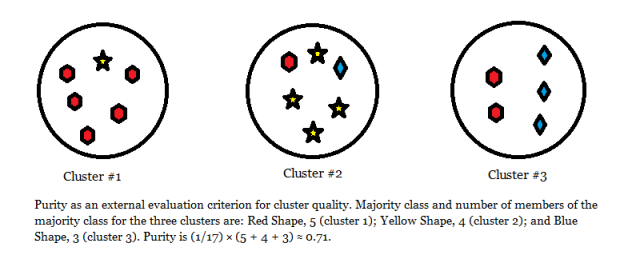
\includegraphics{./Figures/Purityexample.png}
		\rule{35em}{0.5pt}
	\caption[Purity Example]{Purity Example}
	\label{fig:purityFig}
\end{figure}
\subsection{F - Score}
In statistics, the F score (also F-measure) is a measure of a test's accuracy. It considers both the precision $p$ and the recall $r$ of the test to compute the score: $p$ is the number of correct results divided by the number of all returned results and $r$ is the number of correct results divided by the number of results that should have been returned. The F score can be interpreted as a weighted average of the precision and recall, where an F score reaches its best value at 1 and worst score at 0.
The traditional F-measure or balanced F-score (F1 score) is the harmonic mean of precision and recall see equation ~\ref{fmeasure}
\subsection{Confusion Matrix}
An important tool for analyzing the performance of a classifier for $J > 2$ classes is the confusion matrix. The confusion matrix shows for each pair of classes {c1, c2}, how many documents from c1 were incorrectly assigned to c2. It is a specific table layout that allows visualization of the performance of an algorithm. Each column of the matrix represents the instances in a predicted class, while each row represents the instances in an actual class. The name stems from the fact that it makes it easy to see if the system is confusing two classes (i.e. commonly mislabeling one as another). The confusion matrix can help pinpoint opportunities for improving the accuracy of the system. In predictive analytics, a table of confusion (sometimes also called a confusion matrix), is a table with two rows and two columns that reports the number of false positives, false negatives, true positives and true negatives. This allows more detailed analysis. The final table of confusion would contain the average values for all classes combined.

\begin{table}[ht]
\caption{Table of Confusion} % title of Table
\centering  % used for centering table
\begin{tabular}{c c c} % centered columns (5 columns)
\hline\hline                        %inserts double horizontal lines
 & Same Cluster & Different Clusters \\ [0.5ex] % inserts table 
%heading
\hline                  % inserts single horizontal line
Same Class & True Positive (TP)&False Negative (FN)\\ % inserting body of the table
Different Classes & False Positive (FP)& True Negative (TN)  \\[1ex]      % [1ex] adds vertical space
\hline %inserts single line
\end{tabular}
\label{table:conf} % is used to refer this table in the text
\end{table}

From the table of confusion ~\ref{table:conf}, we can calculate Precision, Recall and F-Score as follows:

\begin{equation}
Precision =\frac{TP}{TP + FP}
\end{equation}

\begin{equation}
Recall =\frac{TP}{TP + FN}
\end{equation}

\begin{equation}
\label{fmeasure}
F-Score = 2\times \frac {Recall\times Precision}{Recall + Precision}
\end{equation}

\section{Experiments Design}\label{sec:test}
In this Section we describes how our experiments were performed, what parameters we changed and what variations of modules we used.
Our Experiment is divided to three main variations which are: Lexical-Based Similarity, Semantic Wiki-based Similarity and finally LSA-based Similarity. In each case we compute the $N\times N$ similarities between the documents of the three datasets used.\\
Next we feed these results to our Clustering module based on Mitosis Clustering Technique, where this algorithm takes two parameters as input $(f,k)$ you may refer to section ~\ref{mitosis} for further information.
Finally we try to Cluster the input documents according to the input similarity measure and with various ranges for the Mitosis paramters$(f,k)$, to get the parameters where maximum results are given.

\section{Results and discussion}\label{sec:results}
This section is dedicated for displaying our experiments results, parameter tuning for mitosis and doing some analysis on these results.you can find tables next in this chapter showing the experimental results we have got, where each similarity technique has 2 tables, one for Purity values and the other for F-Score values. This experiment is repeated 2 times for different datasets. you can find these results in tables ~\ref{tables}.\\

Also we used the mean of the obtained purity values to get an overall performace evaluation across various ranges of Mitosis paramters as illustrated in Figures ~\ref{fig:F10}, ~\ref{fig:F11}, ~\ref{fig:F16} \& ~\ref{fig:F30}.\\
Next we provide a simple comparison in Figures ~\ref{fig:F120} \& ~\ref{fig:F121} using the maximum purity measure obtained and Figures  ~\ref{fig:F50} \& ~\ref{fig:F15} using also the maximum obtained F-Score values.

while discussing performace we should mention response time as our techniques running time is slightly larger than that of the pure lexical similarity.Experiments showed that running time of LSA \& Wikipedia approaches ranges from 3.5 - 4 hrs to computer similarity for dataset of size 1000 documents.On the other side the lexical running time was around 2 - 3 hrs, which affect the throughtput. Due to  this costly running time, we couldn't provide more ranges for the experiments.\\

For better and more stable results we have to apply more ranges for the paramter tunning, which their lack may lead to mileading results.This is could be done in future due to lack of time.


\section{Experimental Results}
\label{tables}
\begin{figure}[htbp]
	\centering
		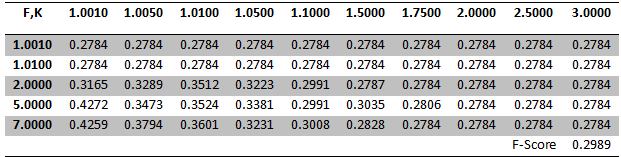
\includegraphics{./Figures/lexical_F_DS1.png}
		\rule{35em}{0.5pt}
	\caption[Mean F-Measure for Lexical Similarity on Dataset one]{Mean F-Measure for Lexical Similarity on Dataset one}
	\label{fig:purity1}
\end{figure}

\begin{figure}[htbp]
	\centering
		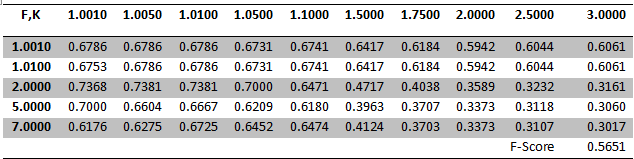
\includegraphics{./Figures/lexical_F_DS2.png}
		\rule{35em}{0.5pt}
	\caption[Mean F-Measure for Lexical Similarity on Dataset Two]{Mean F-Measure for Lexical Similarity on Dataset Two}
	\label{fig:purity2}
\end{figure}

\begin{figure}[htbp]
	\centering
		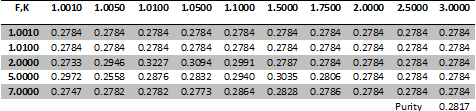
\includegraphics{./Figures/lexical_Purity_DS1.png}
		\rule{35em}{0.5pt}
	\caption[Mean Purity for Lexical Similarity on Dataset one]{Mean Purity for Lexical Similarity on Dataset one}
	\label{fig:purity3}
\end{figure}

\begin{figure}[htbp]
	\centering
		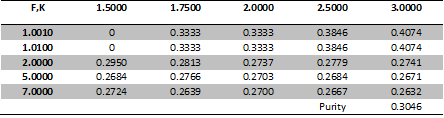
\includegraphics{./Figures/lexical_Purity_DS2.png}
		\rule{35em}{0.5pt}
	\caption[Mean Purity for Lexical Similarity on Dataset two]{Mean Purity for Lexical Similarity on Dataset two}
	\label{fig:purity4}
\end{figure}

\begin{figure}[htbp]
	\centering
		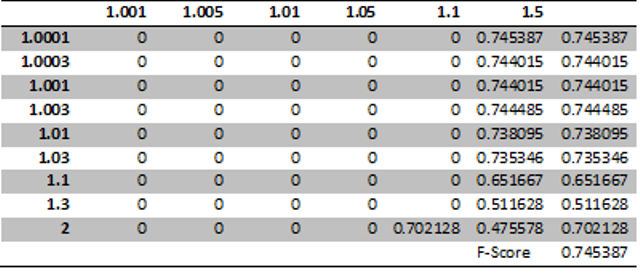
\includegraphics{./Figures/lsa_F_DS1.png}
		\rule{35em}{0.5pt}
	\caption[Mean F-Measure for LSA Similarity on Dataset one]{Mean F-Measure for LSA Similarity on Dataset one}
	\label{fig:F1}
\end{figure}

\begin{figure}[htbp]
	\centering
		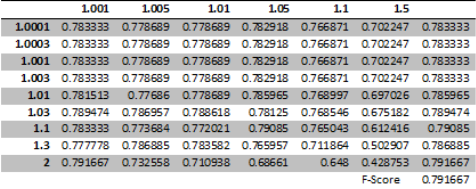
\includegraphics{./Figures/lsa_F_DS2.png}
		\rule{35em}{0.5pt}
	\caption[Mean F-Measure for LSA Similarity on Dataset Two]{Mean F-Measure for LSA Similarity on Dataset Two}
	\label{fig:F2}
\end{figure}

\begin{figure}[htbp]
	\centering
		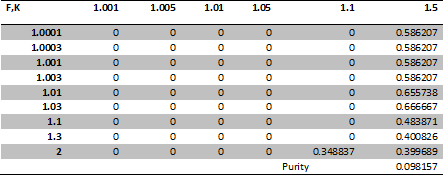
\includegraphics{./Figures/lsa_Purity_DS1.png}
		\rule{35em}{0.5pt}
	\caption[Mean Purity for LSA Similarity on Dataset one]{Mean Purity for LSA Similarity on Dataset one}
	\label{fig:F3}
\end{figure}

\begin{figure}[htbp]
	\centering
		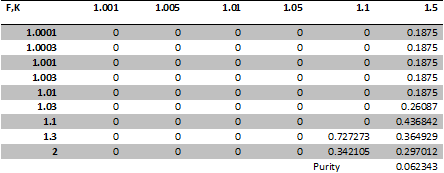
\includegraphics{./Figures/lsa_Purity_DS2.png}
		\rule{35em}{0.5pt}
	\caption[Mean Purity for LSA Similarity on Dataset Two]{Mean Purity for LSA Similarity on Dataset Two}
	\label{fig:F4}
\end{figure}

\begin{figure}[htbp]
	\centering
		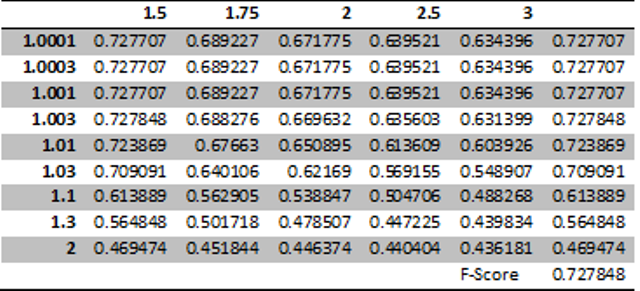
\includegraphics{./Figures/wiki_F_DS1.png}
		\rule{35em}{0.5pt}
	\caption[Mean F-Measure for Wikipedia Similarity on Dataset one]{Mean F-Measure for Wikipedia Similarity on Dataset one}
	\label{fig:F5}
\end{figure}

\begin{figure}[htbp]
	\centering
		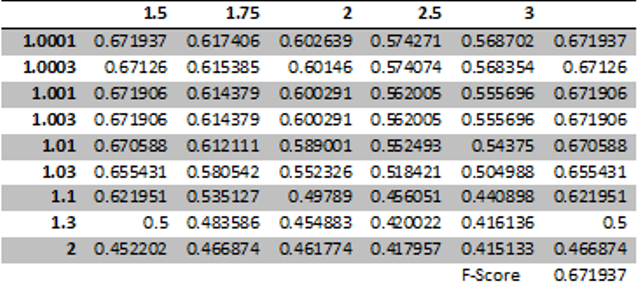
\includegraphics{./Figures/wiki_F_DS2.png}
		\rule{35em}{0.5pt}
	\caption[Mean F-Measure for Wikipedia Similarity on Dataset Two]{Mean F-Measure for Wikipedia Similarity on Dataset Two}
	\label{fig:F6}
\end{figure}

\begin{figure}[htbp]
	\centering
		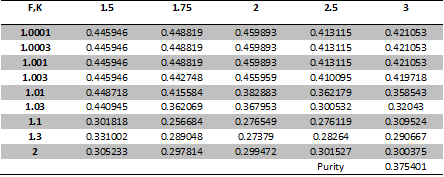
\includegraphics{./Figures/wiki_Purity_DS1.png}
		\rule{35em}{0.5pt}
	\caption[Mean Purity for Wikipedia Similarity on Dataset one]{Mean Purity for Wikipedia Similarity on Dataset one}
	\label{fig:F7}
\end{figure}

\begin{figure}[htbp]
	\centering
		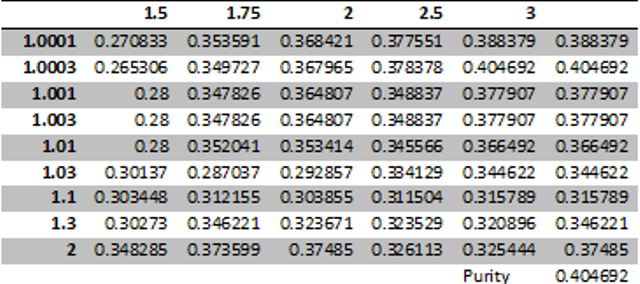
\includegraphics{./Figures/wiki_Purity_DS2.png}
		\rule{35em}{0.5pt}
	\caption[Mean Purity for Wikipedia Similarity on Dataset one]{Mean Purity for Wikipedia Similarity on Dataset Two}
	\label{fig:F8}
\end{figure}
%==================================MEAN=========================================
\begin{figure}[htbp]
	\centering
		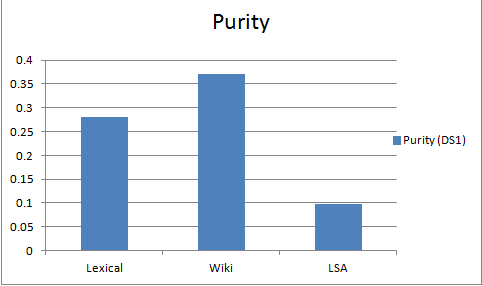
\includegraphics{./Figures/Purity_DS1.png}
		\rule{35em}{0.5pt}
	\caption[Comparison between Purity Mean Values of Different Techniques of Similarity on Dataset one]{Comparison between Purity Mean Values of Different Techniques of Similarity on Dataset one}
	\label{fig:F10}
\end{figure}
\begin{figure}[htbp]
	\centering
		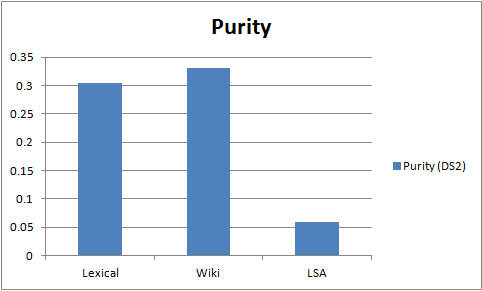
\includegraphics{./Figures/Purity_DS2.png}
		\rule{35em}{0.5pt}
	\caption[Comparison between Purity Mean Values of Different Techniques of Similarity on Dataset Two]{Comparison between Purity Mean Values of Different Techniques of Similarity on Dataset Two}
	\label{fig:F11}
\end{figure}


\begin{figure}[htbp]
	\centering
		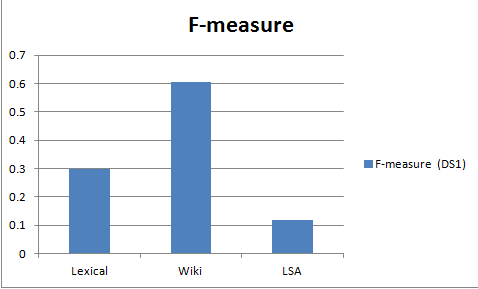
\includegraphics{./Figures/F_DS1.png}
		\rule{35em}{0.5pt}
	\caption[Comparison between Purity Mean Values of Different Techniques of Similarity on Dataset one]{Comparison between Purity Mean Values of Different Techniques of Similarity on Dataset one}
	\label{fig:F16}
\end{figure}
\begin{figure}[htbp]
	\centering
		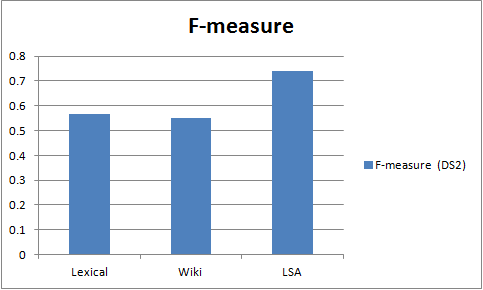
\includegraphics{./Figures/F_DS2.png}
		\rule{35em}{0.5pt}
	\caption[Comparison between Purity Mean Values of Different Techniques of Similarity on Dataset Two]{Comparison between Purity Mean Values of Different Techniques of Similarity on Dataset Two}
	\label{fig:F30}
\end{figure}

%============================MAX==============================
\begin{figure}[htbp]
	\centering
		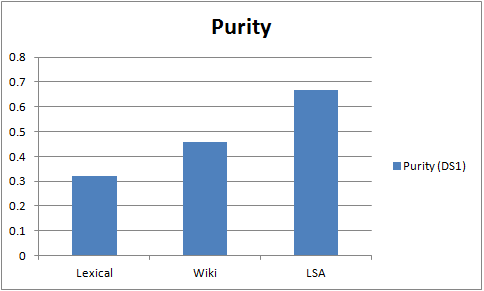
\includegraphics{./Figures/Purity_DS1_1.png}
		\rule{35em}{0.5pt}
	\caption[Comparison between Purity Max. Values of Different Techniques of Similarity on Dataset one]{Comparison between Purity Max. Values of Different Techniques of Similarity on Dataset one}
	\label{fig:F120}
\end{figure}

\begin{figure}[htbp]
	\centering
		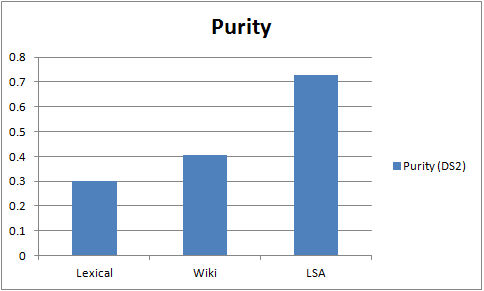
\includegraphics{./Figures/Purity_DS2_1.png}
		\rule{35em}{0.5pt}
	\caption[Comparison between Purity Max. Values of Different Techniques of Similarity on Dataset Two]{Comparison between Purity Max. Values of Different Techniques of Similarity on Dataset Two}
	\label{fig:F121}
\end{figure}
\clearpage
\begin{figure}[htbp]
	\centering
		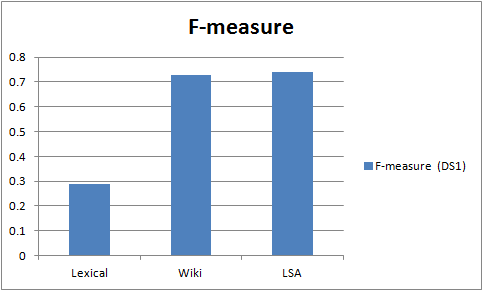
\includegraphics{./Figures/F_DS1_1.png}
		\rule{35em}{0.5pt}
	\caption[Comparison between Purity Max. Values of Different Techniques of Similarity on Dataset one]{Comparison between Purity Max. Values of Different Techniques of Similarity on Dataset one}
	\label{fig:F50}
\end{figure}

\begin{figure}[htbp]
	\centering
		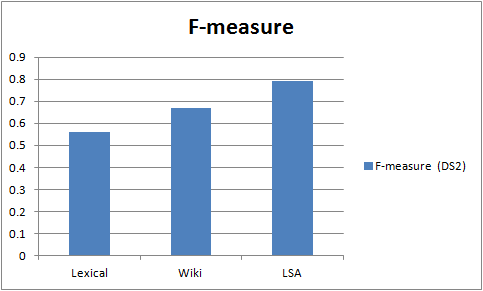
\includegraphics{./Figures/F_DS2_1.png}
		\rule{35em}{0.5pt}
	\caption[Comparison between Purity Max. Values of Different Techniques of Similarity on Dataset Two]{Comparison between Purity Max. Values of Different Techniques of Similarity on Dataset Two}
	\label{fig:F15}
\end{figure}

